\chapter{Die Software-Entwicklung}
\label{chapter3}
Das vorherige Kapitel führte Lehmanns Gesetze ein. Basierend auf deren Annahmen wurden innere und äußere Gründe herausgearbeitet, welche zu diesen Gesetzen führen. Abschließend wurden einige Auswirkungen dieser Gesetze aufgezeigt.\\
In diesem Kapitel wird dargestellt, was Software Modernisierung ist. Dafür wird zunächst der Softwareentwicklungsprozess nach Seacord et al. dargestellt. Anschließend wird die Software-Modernisierung in Seacord’s Entwicklungsprozess  eingeordnet.

\section{Der Software-Entwicklungsprozess}
Die Software-Modernisierung kann als Teil des Software-Entwicklungsprozesses betrachtet werden. 
Seacord et al. \cite{seacord_modernizing_2003} teilt diese in 3 voneinander getrennte Phasen auf.\\
Hierzu zählt zunächst die Instandhaltung der Software. Diese geht über in die Software-Modernisierung. Bis schließlich eine Ersetzung des Systems angestrebt wird. Grafik \ref{fig:lifecycle} illustriert diese 3 Phasen.\\
Die gepunktete Linie in Grafik 3.1 zeigt die Anforderungen der Firma, die sogenannten \textit{Business needs}. Die durchgezogene Linie hingegen gibt die Funktionalität des Systems an.\\
Eine wiederholte Instandhaltung der Software nährt die beiden Linien kurzfristig an. Die Funktionalität ist in diesen Zeitspannen ausreichend um die Business Needs zu befriedigen. 
Mit der Alterung des Systems können zunehmend solche kurzfristigen Lösungen nicht mehr die Funktionalität ausreichend steigern. \\
Eine Modernisierung der Software nimmt mehr Zeit und Geld in Anspruch, als eine Wartung. Mit umfangreichen Änderungen des Systems kann allerdings erneut die Funktionalität an die Anforderungen angeglichen werden. 
Wenn das alte System schließlich nicht mehr weiterentwickelt werden kann, muss es ersetzt werden. 
Die Entscheidung, welche der drei Optionen für ein bestimmtes System angewandt wird, kann nur durch eine eingehende Analyse bestimmt werden. Zeit, Kosten und Abhängigkeiten zur Software sind nur ein kleiner Teil der relevanten Parameter. Oft sind Systemausfälle im Zusammenhang mit längeren Modernisierungsmaßnahmen schlicht nicht akzeptabel. \cite{seacord_modernizing_2003} \\
Im Folgenden werden die Unterschiede von Wartung, Modernisierung und Ersetzung aufgezeigt. 

\begin{figure}[bth] 
  \centering
  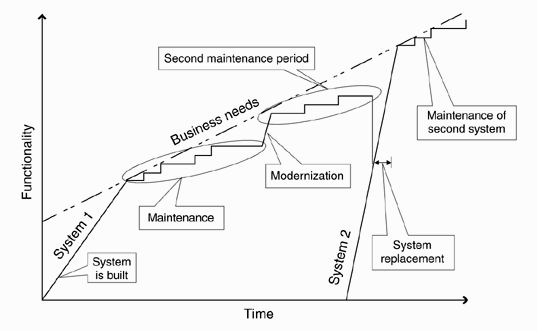
\includegraphics[width=0.7\textwidth]{Chapters/3-Die-Software-Entwicklung/images/LebenszyklusEinesInformationssystems.png}
  \caption{Lebenszyklus eines Informationssystems \cite{seacord_modernizing_2003}}
  \label{fig:lifecycle}
\end{figure}

\section{Software-Wartung}
Die Wartung arbeitet kleine Verbesserungen, wie Fehlerbehebungen oder strukturelle Verbesserungen ein. Diese Anpassungen verändern nichts an der grundsätzlichen Struktur der Software. Folglich bleibt die eigentliche Architektur unangetastet. \cite{seacord_modernizing_2003}\cite{bommer_softwarewartung_2016}\\
\newline
Der Prozess der Wartung ist iterativ. Sie unterstützt die Entwicklung des Systems, hat aber auch Einschränkungen, denn sie erschließt keine Wettbewerbsvorteile. \cite{seacord_modernizing_2003}
Der Umzug in die Cloud oder die Umstellung des Softwareangebots auf Software as a Service sind keine Wartungs-Operationen. Letztere erfordern tiefgreifende strukturelle Anpassungen und können die Architektur des Software-Systems beeinflussen.\\
Allerdings lässt sich die Software-Wartung in Kategorien aufteilen. Diese sind in der Norm IEEE610 festgehalten.:
\begin{description}
    \item [korrektive Wartung] \hfill \\ Boomer et Al. beschreibt diese, als das Beheben von Softwarefehlern. Letztere sind Restfehler, welche nicht während der Entwicklung bemerkt wurden. Die Art des Fehlers kann weiter als Mängel oder Instandhaltung verstanden werden. Ersteres sind kleine Fehler, welche gesammelt und zu gegebener Zeit behoben werden können. Instandhaltung meint allerdings schwere Mängel, welche den Betrieb stören können. \cite{bommer_softwarewartung_2016}
    \item [adaptiver Wartung] \hfill \\ Bei der adaptiven Wartung werden kleine fachliche oder technischen  Anpassungen unternommen. Für erstere wäre die Änderung des Mehrwertsteuersatzes zu nennen. Es kann auf eine neue System-Version umgestellt werden. Diese System-Umstellung ist lediglich dazu da, denn vorherigen Zustand des Systems wiederherzustellen. Hierbei entsteht kein Mehrwert. \cite{bommer_softwarewartung_2016}
    \item [perfektionierender Wartung] \hfill \\ Das Ziel der perfektionierenden Wartung ist die Verbesserung nicht-funktionaler Anforderungen. Mit kleinen Änderungen wird dabei z.B. die Antwortzeit der Software verbessert. \cite{bommer_softwarewartung_2016}
    \item [präventive Wartung] \hfill \\ Bei der präventiven Wartung werden proaktiv Fehler gesucht, welche noch nicht im laufenden Betrieb aufgefallen sind. Diese Tätigkeit ist folglich planbar. \cite{bommer_softwarewartung_2016}
\end{description}
Bommer et Al. \cite{bommer_softwarewartung_2016} kategorisiert diese zudem nach einer reaktiven oder proaktiven Beteiligung. Dies wird in Grafik \ref{fig:proactive} gezeigt. 
\begin{figure}[bth] 
  \centering
  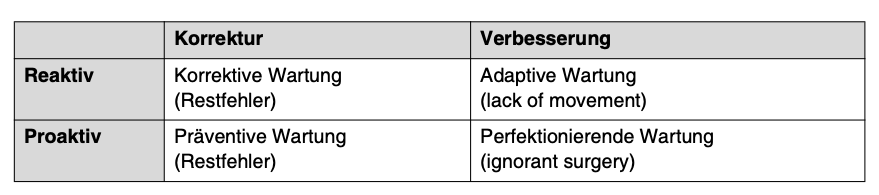
\includegraphics[width=0.7\textwidth]{Chapters/3-Die-Software-Entwicklung/images/KindsOfCorrection.png}
  \caption{Art der Software-Wartung nach proaktiv und reaktiver Beteiligung \cite{bommer_softwarewartung_2016}}
  \label{fig:proactive}
\end{figure}
Darüber hinaus steigt der Schwierigkeitsgrad einer Wartung zunehmend. Denn das Ziel dabei ist es die Software Funktionalitäten erneut an die Business Needs anzupassen. Strukturelle Verbesserungen und Fehlerbehebungen genügen dafür, bei einer stark gewachsenen Software, nicht mehr.

\section{Software-Modernisierung}
Die Software-Modernisierung ist der Prozess der Weiterentwicklung einer Software. Dies geschieht, indem Teile ersetzt, neu-entwickelt oder auf eine neue Plattform migriert werden. \cite{khadka_does_2015}
Khadka et Al. \cite{ravi_khadka_how_nodate} nennt die zu modernisierenden Systeme \glqq[...] Legacy Systems [...]\grqq{}, sofern diese schwer anzupassen sind und dennoch kritisch sind für das laufende Geschäft. Die Software-Modernisierung passt Legacy-Systeme an gewachsene System-Anforderungen an, wenn dies nicht mehr durch Wartungsmaßnahmen getan werden kann. Daraus ergibt sich, dass die Software-Modernisierung dann eingesetzt wird, wenn eine Wartung zu schwierig und kostspielig ist. \\
Die Software-Modernisierung arbeitet dabei größere Änderungen in das System ein. Zu beachten ist allerdings, dass ein Großteil des Systems beibehalten wird. Dies ist dann von Nutzen, wenn ein Software-System Anpassungen benötigt. Allerdings der Kern des Systems weiterhin ein Business Value hat. \cite{seacord_modernizing_2003}\\
Seastorm et Al. \cite{seacord_modernizing_2003} unterscheidet zudem \textit{White-Box Modernisierung} und \textit{Blackbox Modernisierung}. Die White-Box Modernisierung benötigt wissen über die internen Komponenten.  Wohingegen Black-Box Modernisierung nur Kenntnisse über externe Schnittpunkte benötigt. 

\section{Software-Neuentwicklung}
Die Neuentwicklung benötigt den Aufbau eines komplett neuen Software-Systems. Folglich ist dieser Ansatz kosten- und zeit-intensiv. 
Die Software-Neuentwicklung bietet sich an, wenn sowohl White-Box, als auch Black-Box Modernisierung nicht kostengünstiger als die Neuentwicklung sind.\\
Hier ist anzumerken, dass nicht alle Bestandteile des Systems gleichzeitig erneuert werden müssen. Eine Architektur bestehend aus klar abgetrennten Systemen kann auch teilweise neu entwickelt werden. \\
In diesem Stadium gilt zu evaluieren, ob eine kommerzielle Software für die gegebenen Anforderungen geeignet ist. Diese sogenannte \ac{COTS} Software \cite{abts_cocots_2000} sind in unter anderem als Customer-Resource-Management-Systeme oder Finanz-Systeme verfügbar. 
\acs{COTS} Software-Systeme sind bereits fertig implementierte Software-Bausteine für die genannten Anwendungsfälle. Eine firmeneigene Entwicklung kann so vermieden werden. \cite{abts_cocots_2000}\cite{seacord_modernizing_2003}





